\chapter{Specialising and optimising xDSL pattern rewriting}
\label{chap:specialising-optimising-pattern-rewriting}

%% Introduction and goals (make faster and only constrained by language runtime)
% Hook
In \autoref{chap:measuring-compiler-performance}, we constructed a set of experiments to empirically compare the current performance of the xDSL and \ac{mlir} compiler frameworks.
% Argument
Our overall aim is to use these experiments to contrast the performance of static and dynamic languages for the implementation of user-extensible compiler frameworks, using \ac{mlir} and xDSL as proxies for these two categories respectively.
However, the experiments so far measure a combination of the effects of dynamism in the language runtime and implementation details of the framework, with the former obscuring our goal of measuring the latter.
% Link
In order to use the frameworks for our aims, our measurements must be as independent of implementation details as possible.

% Hook
In this chapter, we meet this requirement by specialising the xDSL framework to implement only a single workload.
% Argument
In this process, we manually identify and remove computation performed by the framework which is unnecessary to its execution of this workload. One common example of this is functionality which improves the expressivity of the framework, such as runtime type checks to support polymorphism of arguments. A second example is calculating and checking values which are known as runtime invariants for the selected workload, such as checking properties of empty fields.
% In this process, we manually identify and remove computation performed by the framework which is unnecessary to its execution of this workload. This computation broadly falls into two categories. The first is functionality which improves the expressivity of the framework, such as runtime type checks to support polymorphism of arguments. The second is calculating and checking values which are known as runtime invariants for the selected workload. % DONE: Does it make sense to split these into categories, almost the same thing in some sense -- no!
By eliminating these performance overheads, we reach an implementation representative of the best-case performance of Python for this workload.
% Link
The benefits of this specialisation are twofold. Firstly it reveals inefficiencies in xDSL which can be optimised to improve the general performance of the framework. Secondly, it provides a true performance baseline for dynamic languages irrespective of implementation details which can be used to quantify the impact of dynamism in \autoref{chap:dynamism-pattern-rewriting}.


\section{Micro-benchmarks}
\label{sec:specialising-ubenchmarks}

%% Link back to micro-benchmarks and summarise section
% Hook
An important component of our experimental suite is micro-benchmarks, measuring the performance of procedures fundamental to xDSL and \ac{mlir}.
% Argument
The small size of these micro-benchmarked procedures makes them tractable first targets for manual specialisation and optimisation, with the performance impact of this process easily characterised by repeating the micro-benchmark.
By manually examining the traces of their execution, we can identify and eliminate any unnecessary computation in the current implementation.
% Link
Having done this, we re-run the micro-benchmarks to quantify the performance of the specialised implementation, facilitating comparison of the language runtime only for user-extensible compiler framework workloads.
% In this section, we examine the specialisation process for these micro-benchmarks in detail. % TODO: Add more stuff here!!


\subsection{Operation instantiation}
\label{sec:specialising-ubenchmarks-instantiation}

%% Re-introduce microbenchmark
% Hook
The first micro-benchmark discussed in \autoref{sec:ubenchmark} was instantiating operations, one of the central data structures in both xDSL and \ac{mlir}.
% Argument
The idiomatic way to do this in xDSL is directly instantiating a new Python object.
This invokes the \mintinline{text}{__new__} method to construct an empty class, then the \mintinline{text}{__init__} method to initialise it, and optionally \mintinline{python3}{__post_init__} following initialisation.
In xDSL, this instantiation process includes a large amount of logic (\autoref{fig:ubenchmark-original-instantiation-xdsl-viztracer}), including verifying attributes and building properties of the operation.
However, in many instances this verification is unneeded as it is already known as a runtime invariant, and the building process can similarly be simplified as the structure can be inferred.
% Link
As such, specialisation to remove this overhead can vastly reduce the complexity and hence improve performance (\autoref{fig:ubenchmark-optimised-instantiation-xdsl-viztracer}).

\begin{figure}[H]
    \centering
    \begin{subfigure}[b]{\textwidth}
        \centering
        \begin{tikzpicture}
            \node[anchor=south west,inner sep=0] (image) at (0,0) {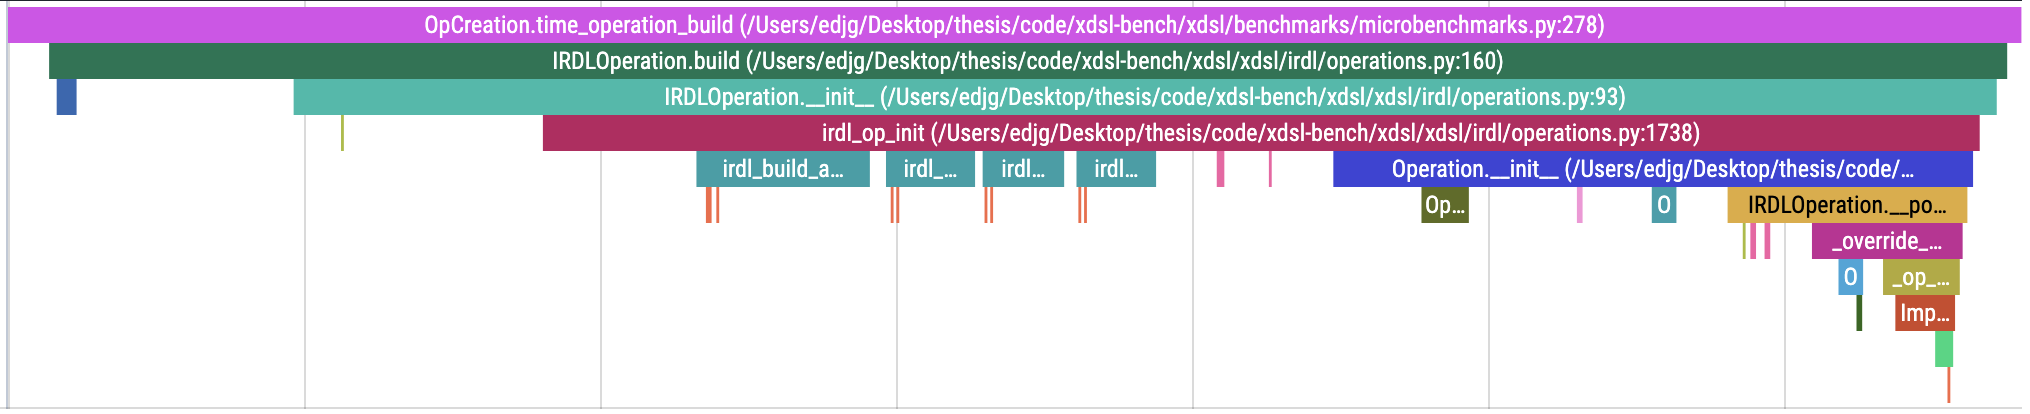
\includegraphics[width=\textwidth]{images/specialising_optimising_xdsl_rewriting/original_empty_create}};
            \node[circledstyle, fill=pairedOneLightBlue] at (6.25,1.25) {A};
            \node[circledstyle, fill=pairedTwoDarkBlue] at (14,0.75) {B};
        \end{tikzpicture}
        \captionsetup{width=0.8\textwidth}
        \caption{The default constructor has a high overhead, calculating known invariants and .}
        \label{fig:ubenchmark-original-instantiation-xdsl-viztracer}
    \end{subfigure}
    \begin{subfigure}[b]{\textwidth}
        \centering
        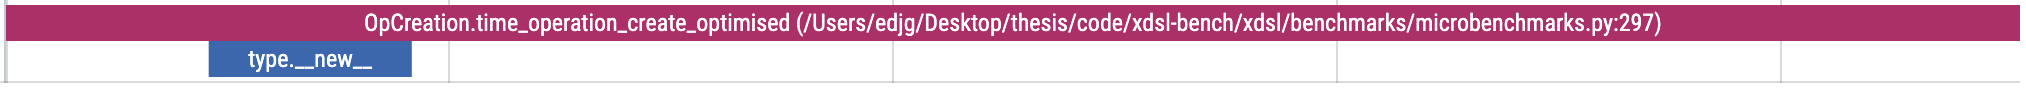
\includegraphics[width=\textwidth]{images/specialising_optimising_xdsl_rewriting/optimised_empty_create}
        \captionsetup{width=0.8\textwidth}
        \caption{The same object can be constructed with significantly less logic.}
        \label{fig:ubenchmark-optimised-instantiation-xdsl-viztracer}
    \end{subfigure}
    \caption{\texttt{viztracer} traces of xDSL instantiating an \texttt{EmptyOp} before (top) and after (bottom) specialisation.}
    \label{fig:ubenchmark-instantiation-xdsl-viztracer}
\end{figure}

%% Describe specialisation/optimisation
% Hook
Examining the above trace, we can visually identify components which take a large proportion of runtime, and may represent unnecessary computation.
% Argument
For example, the xDSL constructor for \mintinline{python3}{IRDLOperation}s invokes logic with significant overhead building and filtering properties of the operation \circledbase{pairedOneLightBlue}{A}. However, in this example of the empty operation, this logic does not change the constructed object. Because of this, eliding this logic results in a specialised version of the operation which generates the same output using less computation by applying domain knowledge.
In addition to this, \ac{mlir}'s core operations are not \ac{irdl} based, unlike xDSL, meaning this overhead is implementation specific.
Similarly, the post-constructor includes logic for context-managed builders \circledbase{pairedTwoDarkBlue}{B}, which is again unrelated to the empty operation case and not present in \ac{mlir}.
% Link
To avoid this overhead through specialisation, we move from the idiomatic constructor (Listing \ref{listing:ubenchmark-xdsl-constant-constructor}) to directly modifying xDSL's underlying data structures (Listing \ref{listing:ubenchmark-xdsl-constant-direct}).


\begin{figure}[H]
    \begin{subfigure}[b]{0.5\textwidth}
       \centering
        \begin{minted}[fontsize=\footnotesize]{text}
            EmptyOp()
        \end{minted}
        \footnotesize\vspace{4em}
        \caption{Instantiation with constructors.}
        \label{listing:ubenchmark-xdsl-constant-constructor}
    \end{subfigure}
    \hfill
    \begin{subfigure}[b]{0.5\textwidth}
        \centering
        \begin{minted}[breakanywhere,fontsize=\footnotesize]{text}
            empty_op = EmptyOp.__new__(EmptyOp)
            empty_op._operands = tuple()
            empty_op.results = tuple()
            empty_op.properties = {}
            empty_op.attributes = {}
            empty_op._successors = tuple()
            empty_op.regions = tuple()
        \end{minted}
        \caption{Instantiation by direct manipulation of xDSL's data structures.}
        \label{listing:ubenchmark-xdsl-constant-direct}
    \end{subfigure}
    \captionsetup{name=Listing}
    \caption{Approaches to instantiating an empty operation.}
    \label{listing:ubenchmark-xdsl-constant}
\end{figure}

%% Specialised performance and lessons learnt
% Hook
Through specialising the implementation to the workload of this micro-benchmark we can achieve significant performance improvements of up to $26\times$ (\autoref{tab:ubenchmark-instantiation-optimised}).
% Argument
% Drop runtime by performing fewer, quicker operations
We can quantify the one cause of this improvement by leveraging our novel bytecode profiling tool as the specialised code executing fewer, faster bytecode instructions (Listing \ref{listing:bytecode-profiles-op-build-original}, Listing \ref{listing:bytecode-profiles-op-build-optimised}).
For example, specialisation reduces the number of instructions executed from $466$ to only $29$. Of these instructions, function calls occupy a disproportionate amount of runtime, with their mutation of the call stack taking up to three times longer than other operations such as loading variables. Again leveraging our tool, we can see that specialisation reduces the number of function calls from $65$ to $5$, further improving performance.
% This process comes with the drawback of making the API much more complex
However, the performance improvement comes at the cost of a significantly more complex implementation, contrary to xDSL's design goaals of a simple expressive API.
% close to MLIR

% TODO: Might need stronger argument of approximate optimality from bytecode trace?

%% Compare performance
\begin{table}[H]
  \caption{.}
  \label{tab:ubenchmark-instantiation-optimised}
  \centering
  \begin{tabular}{ccc}
    \toprule
    \textbf{MLIR [ns]} & \textbf{xDSL [ns]} & \textbf{Optimised xDSL [ns]} \\
    \midrule
    $153 \pm 0.5$ & $12700 \pm 1810$ & $477 \pm 385$ \\
    \bottomrule
  \end{tabular}
\end{table}


% %% Doesn't exactly match MLIR, because dynamism means it doesn't incur heavy RTTI machinery
% % TODO: Move this into dynamism section!!!!!!!
% % Hook
% The specialised implementation achieves a slowdown of only $3\times$ from \ac{mlir}, which is surprising...
% % Argument
% % Link
% Despite this, the specialised implementation approaches the upper bound of performance for this workload as a result of the constraints of the language runtime, making it suitable for the comparison of dynamic and static language runtimes.







\subsection{Operation trait checks}
\label{ssec:specialising-ubenchmarks-trait}

%% Re-introduce microbenchmark
% Hook
The second micro-benchmark discussed involved checking traits on operations, and was measured to perform $80\times$ worse in xDSL than \ac{mlir}.
% Argument
Similarly to the operation instantiation micro-benchmark, this slow-down results from a high proportion of method's logic not implementing the core functionality (\autoref{fig:ubenchmark-hastrait-original-viztracer}). In this case, this logic improves the expressivity of the API, supporting both concrete objects and types as arguments, along with handling the edge case of unregistered operations. However, this logic lies on the hot path of execution, and again these properties are known as runtime invariants. As such, specialisation can again be leveraged to remove this implementation overhead (\autoref{fig:ubenchmark-hastrait-optimised-viztracer}).
% Link

\begin{figure}[H]
    \centering
    \begin{subfigure}[b]{\textwidth}
        \centering
        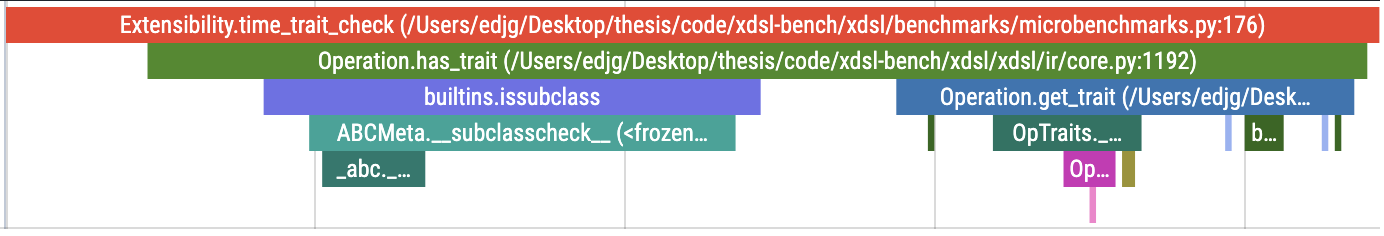
\includegraphics[width=\textwidth]{images/specialising_optimising_xdsl_rewriting/original_hastrait.png}
        \captionsetup{width=0.8\textwidth}
        \caption{\mintinline{python}{issubclass} and \mintinline{python}{isinstance} checks, type \mintinline{python}{cast}ing, and constructing iterators constitutes over three quarters of xDSL's \mintinline{python}{has_trait}s runtime.}
        \label{fig:ubenchmark-hastrait-original-viztracer}
    \end{subfigure}
    \begin{subfigure}[b]{\textwidth}
        \centering
        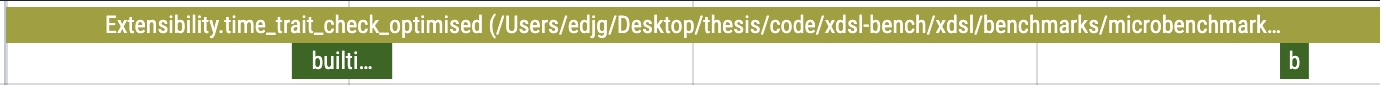
\includegraphics[width=\textwidth]{images/specialising_optimising_xdsl_rewriting/optimised_hastrait.png}
        \captionsetup{width=0.8\textwidth}
        \caption{Specialisation to narrow the interface and optimisation to avoid extraneous work on hot paths can significantly accelerate \mintinline{python}{has_trait}.}
        \label{fig:ubenchmark-hastrait-optimised-viztracer}
    \end{subfigure}
    \caption{\texttt{viztracer} traces of xDSL's \mintinline{python}{has_trait} method.}
    \label{fig:ubenchmark-hastrait-viztracer}
\end{figure}

%% Describe specialisation/optimisation
% Hook
Examining the implementation of this micro-benchmark (Listing \ref{listing:ubenchmark-trait-checks-xdsl}), we can again identify opportunities for specialisation and optimisation.
% Argument
The execution trace shows that checking the whether an operation is unregistered  $\circledbase{pairedOneLightBlue}{1}$ accounts for over one third of the micro-benchmark runtime. Through specialisation under the runtime invariant that all operations are registered, this check can be removed -- reducing computation. Furthermore, this inspires a general optimisation to xDSL to avoid this check by overloading \mintinline{python}{UnregisteredOp.has_trait} rather than checking on all code paths.
In addition to this, function invocation in Python incurs a performance cost due to the overhead of modifying the stack frame. As such, inlining the call to \mintinline{python}{get_trait} \circledbase{pairedTwoDarkBlue}{2} is another beneficial specialisation.
Finally, argument types are dynamically checked \circledbase{pairedThreeLightGreen}{3} and casted \circledbase{pairedFourDarkGreen}{4}, incurring a performance overhead. However, the type of these arguments are runtime invariants of the caller, so the checks can be specialised away.
% Link

\begin{figure}[H]
    \begin{subfigure}[b]{0.45\textwidth}
       \centering
        \begin{minted}[fontsize=\footnotesize,escapeinside=££]{text}
            @classmethod
            def has_trait(
                cls,
                trait: type[OpTrait] | OpTrait,
                *,
                value_if_unregistered: bool = True,
            ) -> bool:
                from xdsl.dialects.builtin import UnregisteredOp £\circledbase{pairedOneLightBlue}{1}£
                if issubclass(cls, UnregisteredOp):
                    return value_if_unregistered

                return cls.get_trait(trait) is not None £\circledbase{pairedTwoDarkBlue}{2}£
        \end{minted}
        \footnotesize\vspace{1.5em}
        \caption{Outer \mintinline{python}{has_trait} method.}
        \label{listing:ubenchmark-trait-checks-xdsl-has}
    \end{subfigure}
    \hfill
    \begin{subfigure}[b]{0.45\textwidth}
        \centering
        \begin{minted}[breakanywhere,fontsize=\footnotesize,escapeinside=££]{text}
            @classmethod
            def get_trait(
                cls,
                trait: type[OpTraitInvT] | OpTraitInvT
            ) -> OpTraitInvT | None:
                if isinstance(trait, type): £\circledbase{pairedThreeLightGreen}{3}£
                    for t in cls.traits:
                        if isinstance(t, cast( £\circledbase{pairedFourDarkGreen}{4}£
                            type[OpTraitInvT], trait
                        )):
                            return t
                else:
                    for t in cls.traits:
                        if t == trait:
                            return cast(OpTraitInvT, t)
                return None
        \end{minted}
        \caption{Inner \mintinline{python}{get_trait} method.}
        \label{listing:ubenchmark-trait-checks-xdsl-get}
    \end{subfigure}
    \vspace{1em}
    \captionsetup{name=Listing}
    \caption{xDSL methods implementing trait check functionality.}
    \label{listing:ubenchmark-trait-checks-xdsl}
\end{figure}

%% Understand specialisation
% Hook
Having specialised xDSL's implementation, we can draw direct comparison between its implementation (Listing \ref{listing:ubenchmark-trait-checks-both-xdsl}) and MLIR's (Listing \ref{listing:ubenchmark-trait-checks-both-mlir}), to better understand their relative performance characteristics.
% Argument
In contrast to the original, the specialised implementation directly matches \ac{mlir}, with the only difference being the mechanism by which traits are checked.
% Link
As such, it is well-suited for comparing the performance characteristics of static and dynamic languages independent of implementation details.

\begin{figure}[H]
    \centering
    \begin{subfigure}[b]{0.45\textwidth}
       \centering
        \begin{minted}[fontsize=\footnotesize]{text}
            for t in OP.traits._traits:
                if isinstance(t, TRAIT):
                    return True
            return False
        \end{minted}
        \footnotesize\vspace{2em}
        \captionsetup{name=Listing}
        \caption{xDSL's modified \mintinline{python}{has_trait} method.}
        \label{listing:ubenchmark-trait-checks-both-xdsl}
    \end{subfigure}
    \hfill
    \begin{subfigure}[b]{0.45\textwidth}
        \centering
        \begin{minted}[breakanywhere,fontsize=\footnotesize]{text}
            TypeID traitIDs[] = {TypeID::get<Traits>()...};
            for (unsigned i = 0, e = sizeof...(Traits); i != e; ++i)
                if (traitIDs[i] == traitID)
                    return true;
            return false;
        \end{minted}
        \captionsetup{name=Listing}
        \caption{\ac{mlir}'s \mintinline{c++}{has_trait} method.}
        \label{listing:ubenchmark-trait-checks-both-mlir}
    \end{subfigure}
    \vspace{1em}
    \captionsetup{name=Listing}
    \caption{xDSL and \ac{mlir} methods searching trait arrays.}
    \label{listing:ubenchmark-trait-checks-both}
\end{figure}

%% Specialised performance and lessons learnt
% Hook
Through specialisation, we achieve a $3.5\times$ speedup over the original implementation (\autoref{fig:ubenchmark-original-trait-performance}).
% Argument
This speedup is less dramatic than operation instantiation, as a result of having less overhead in the original implementation, but can be reasoned about in the same manner with our novel profiling tool. As before, specialisation reduces the number of bytecode instructions from $89$ to $35$, with the number of high-overhead \texttt{CALL} instructions dropping from $11$ to $2$.
% In addition to this, the similarity of the two implementations allows us to draw comparisons between the bytecode and assembly instructions
However, this again incurs a cost to xDSL's expressivity, sacrificing polymorphic support for checking traits of both object types and instances. As with operation instantiation, this is contrary to xDSL's design goals. % TODO: Close more neatly!
% Link

% TODO: Might need stronger argument of approximate optimality from bytecode trace?

%% Compare performance and number of bytecode/assembly operations
\begin{figure}[H]
    \centering
    \begin{subfigure}[b]{0.45\textwidth}
        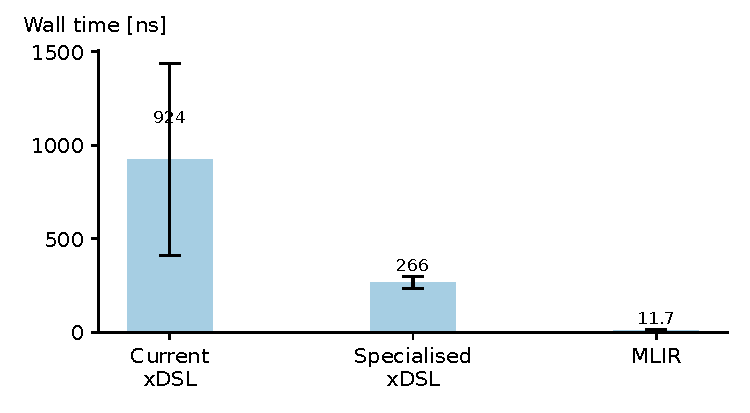
\includegraphics[width=\textwidth]{images/specialising_optimising_xdsl_rewriting/trait_performance.pdf}
        \caption{.}
        \label{fig:ubenchmark-original-trait-performance}
    \end{subfigure}
    \hfill
    \begin{subfigure}[b]{0.45\textwidth}
        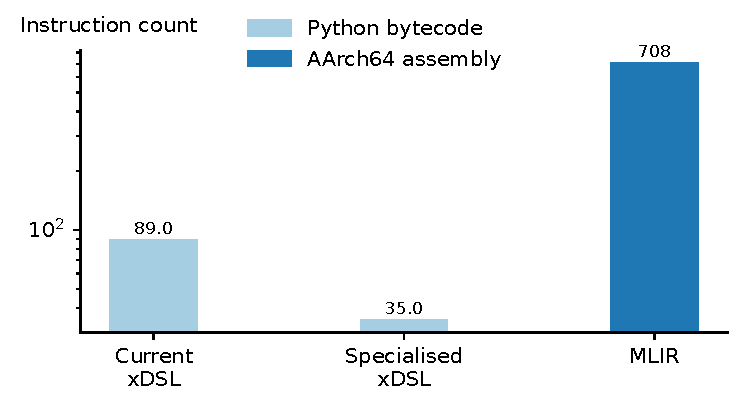
\includegraphics[width=\textwidth]{images/specialising_optimising_xdsl_rewriting/trait_instructions.pdf}
        \caption{.}
        \label{ubenchmark-original-trait-instructions}
    \end{subfigure}
    \caption{.}
    \label{ubenchmark-original-trait-summary}
\end{figure}







%% ======================================================== %%
%% This subsection would just repeat the points made above? %%
%% ======================================================== %%
% \subsection{What does specialisation do?}
% \label{ssec:specialising-what-do}
% %% What does specialisation do
% % Hook
% From the above two micro-benchmarks, we have empirically demonstrated that specialisation to workloads improves their performance, approaching the best-case .
% % Argument
% The mechanism for this is simple: specialisation uses extra information in the form of runtime invariants to avoid work at runtime, reducing the number of bytecode instructions the interpreter needs to execute.
% % Relate into JIT compilation and stuff
% % Link
% Having demonstrated and understood the effectiveness of specialisation for small workloads, we can now leverage it for a non-trivial example of pattern rewriting.
%% Summary table??
% \begin{table}[H]
% %   \caption{Specialisation improves xDSL's operation instantiation performance by $26\times$, lifting it from $83\times$ to $3\times$ slower than \ac{mlir}.}
%   \caption{Specialisation improves xDSL's performance for micro-benchmarks.}
%   \label{tab:ubenchmark-instantiation-optimised}
%   \centering
%   \begin{tabular}{cccc}
%     \toprule
%     \textbf{} & \textbf{MLIR [ns]} & \textbf{xDSL [ns]} & \textbf{Specialised xDSL [ns]} \\
%     \midrule
%     Operation instantiation & $153 \pm 0.5$ & $12700 \pm 1810$ & $477 \pm 385$ \\
%     % Operation instantiation & $357 \pm 0.5$ & $33400 \pm 3680$ & $1830 \pm 774$ \\
%     Trait checking & $11.7 \pm 0.5$ & $924 \pm 513$ & $266 \pm 34$\\
%     \bottomrule
%   \end{tabular}
% \end{table}







\section{Pattern rewriting}
\label{sec:specialising-pattern-rewriting}

%% Introduce actual workload over micro-benchmarks
% Hook
Having demonstrated specialisation as an approach to approach the performance bound of a language for micro-benchmarks%to examine the underlying language runtime performance for micro-benchmarks
, we can further apply it to real-world workloads such as constant folding.
% Argument
In this section, we specialise a simple pattern rewriter: constant folding over integer add operations. Unlike previous micro-benchmarks, MLIR's implementation of pattern rewriting also introduces non-negligible implementation overhead. As such, we provide a matching implementation of this algorithm in MLIR to guarantee fair comparison.
% Link
These specialised implementations can then be taken as performance baselines for their respective languages, and further analysed through bytecode tracing or disassembly to understand their implementation.


\subsection{Constant folding workload}
\label{sec:specialising-pattern-rewriting-workload}

%% Summarise the workload and how it is special (xDSL and MLIR!)
% Hook
% Argument
% Link

%% Listing showing the two guys
\begin{figure}[H]
    \centering
    \begin{subfigure}[b]{0.45\textwidth}
       \centering
        \begin{minted}[fontsize=\scriptsize]{python}
def match_and_rewrite(self, op: Operation, rewriter: PatternRewriter, /):
    # Only rewrite integer add operations
    if not isinstance(op, AddiOp):
        return

    # Ensure both operands are constants
    lhs_op = op.operands[0].op
    rhs_op = op.operands[1].op
    assert lhs_op.has_trait(ConstantLike)
    assert rhs_op.has_trait(ConstantLike)

    # Calculate the result of the addition
    lhs = lhs_op.value.value.data
    rhs = rhs_op.value.value.data
    folded_op = ConstantOp(
        IntegerAttr(lhs + rhs, op.result.type)
    )

    # Rewrite with the calculated result
    rewriter.replace_matched_op(
        folded_op, [folded_op.results[0]]
    )
        \end{minted}
        \footnotesize\vspace{5em}
        \captionsetup{name=Listing}
        \caption{xDSL implementation.}
        \label{listing:constant-folding-impl-xdsl}
    \end{subfigure}
    \hfill
    \begin{subfigure}[b]{0.5\textwidth}
        \centering
        \begin{minted}[breakanywhere,fontsize=\scriptsize]{c++}
  // Only rewrite integer add operations
  LogicalResult matchAndRewrite(arith::AddIOp op, PatternRewriter &rewriter) const override {

    // Ensure both operands are constants
    arith::ConstantOp lhsConstOp = op.getLhs().getDefiningOp<arith::ConstantOp>();
    arith::ConstantOp rhsConstOp = op.getRhs().getDefiningOp<arith::ConstantOp>();
    if (!lhsConstOp || !rhsConstOp) {
        return failure();
    }

    // Calculate the result of the addition
    auto lhsAttr = lhsConstOp.getValue().dyn_cast<IntegerAttr>();
    auto rhsAttr = rhsConstOp.getValue().dyn_cast<IntegerAttr>();
    if (!lhsAttr || !rhsAttr) {
        return failure();
    }
    APInt lhsValue = lhsAttr.getValue();
    APInt rhsValue = rhsAttr.getValue();
    APInt result = lhsAttr.getValue() + rhsAttr.getValue();

    // Rewrite with the calculated result
    auto resultType = op.getType();
    auto foldedValue = rewriter.getIntegerAttr(resultType, result);
    rewriter.replaceOpWithNewOp<arith::ConstantOp>(op, resultType, foldedValue);
    return success();
  }
        \end{minted}
        \captionsetup{name=Listing}
        \caption{\ac{mlir} implementation.}
        \label{listing:constant-folding-impl-mlir}
    \end{subfigure}
    \vspace{1em}
    \captionsetup{name=Listing}
    \caption{Implementations of constant folding over integer addition.}
    \label{listing:constant-folding-impl}
\end{figure}


\subsection{Specialisation}
\label{sec:specialising-pattern-rewriting-specialisation}

%% What does specialisation mean in this context (inlining/eliding/...)
Due to the length of the constant folding workload, there are many more opportunities for specialisation than in the above micro-benchmarks. Despite this, the overall approach is the same: removing unnecessary computation
% Link
% Argument
% Link

%% Figure comparing traces

\begin{figure}[H]
    \centering
    \begin{subfigure}[b]{\textwidth}
        \centering
        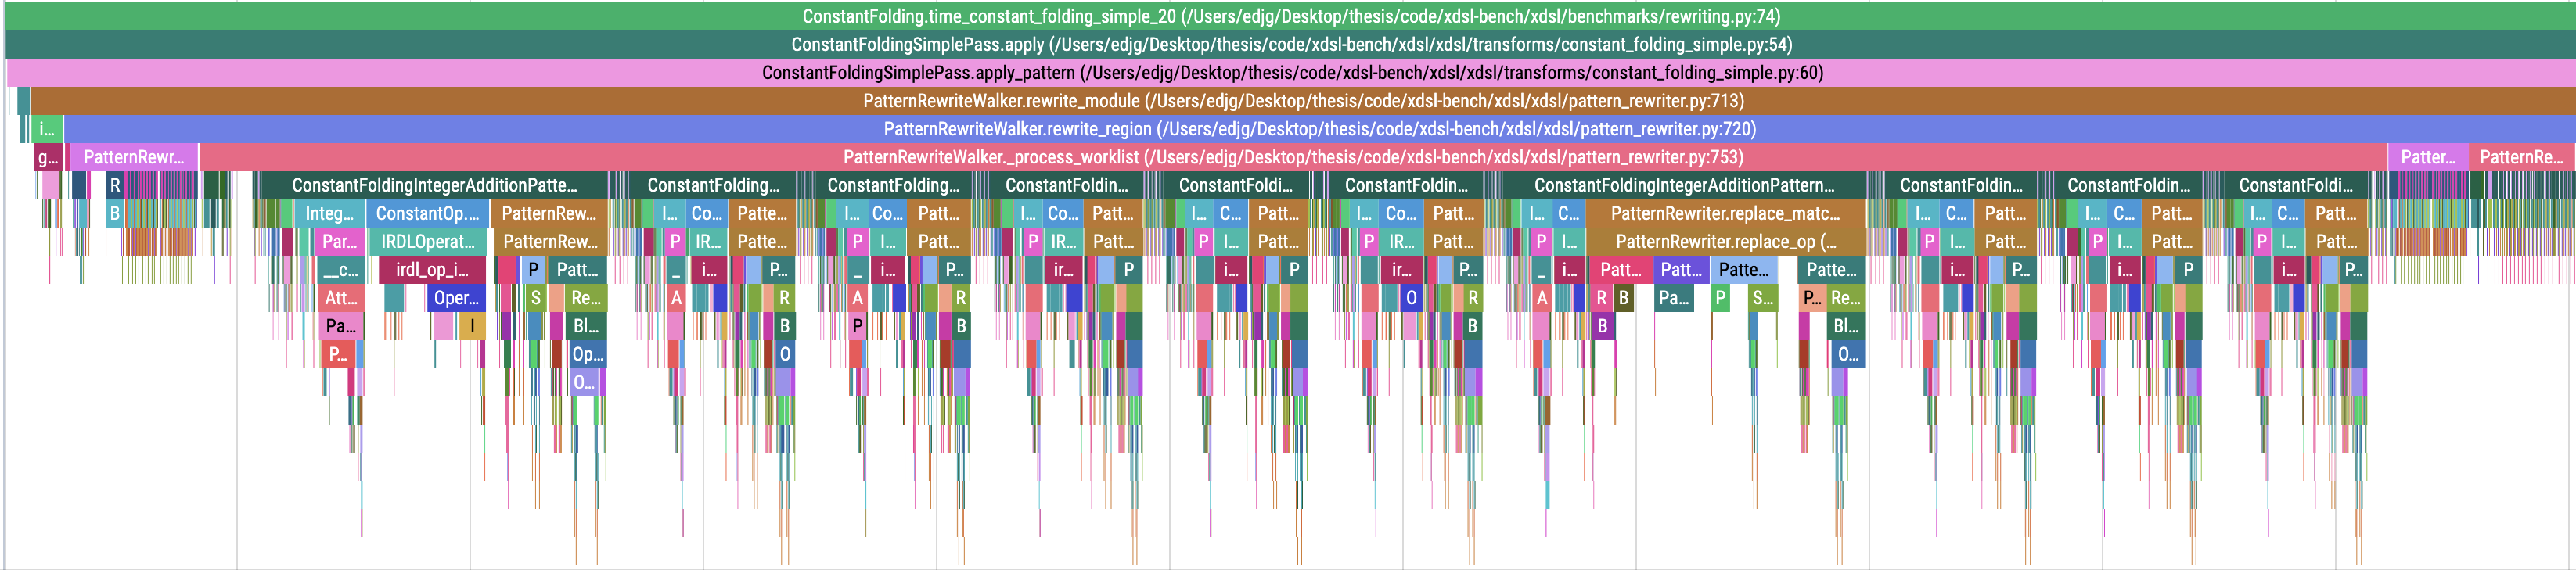
\includegraphics[width=\textwidth]{images/specialising_optimising_xdsl_rewriting/custom_constant_fold.png}
        \captionsetup{width=0.8\textwidth}
        \caption{.}
        \label{fig:constant-fold-original-viztracer}
    \end{subfigure}
    \begin{subfigure}[b]{\textwidth}
        \centering
        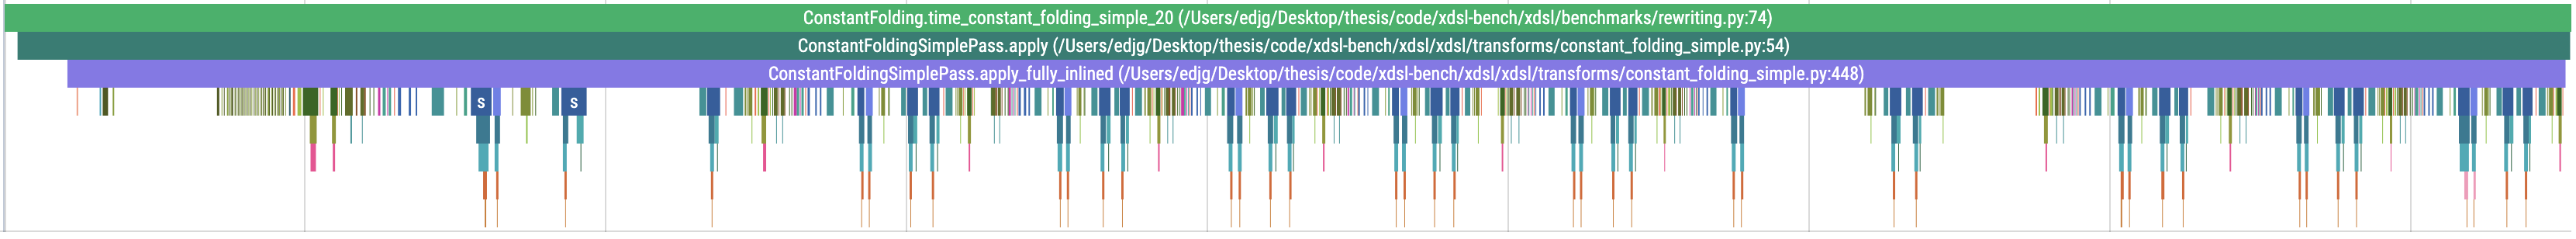
\includegraphics[width=\textwidth]{images/specialising_optimising_xdsl_rewriting/optimised_constant_fold.png}
        \captionsetup{width=0.8\textwidth}
        \caption{.}
        \label{fig:constant-fold-optimised-viztracer}
    \end{subfigure}
    \caption{\texttt{viztracer} traces of.}
    \label{fig:constant-fold-viztracer}
\end{figure}

%% Either perf table here or later in summary?

%% Hopes of automation?
% Link
% Argument
% Link

\subsection{Performance improvement}
\label{sec:specialising-pattern-rewriting-performance}

%% How much did we get out of this?
% Link
% Argument
% Link

%% Figure or table comparing performance
\begin{table}[H]
  \caption{.}
  \label{tab:constant-folding-optimised}
  \centering
  \begin{tabular}{ccc}
    \toprule
    \textbf{MLIR [ns]} & \textbf{xDSL [ns]} & \textbf{Optimised xDSL [ns]} \\
    \midrule
    $3.89 \pm 0.01$ & $504 \pm 76$ & $63.6 \pm 40$\\
    \bottomrule
  \end{tabular}
\end{table}
% Test ConstantFoldingSimple.20(unspecialised) ran in: 0.00115 ± 3e-05s
% Test ConstantFoldingSimple.20(unspecialised) ran in: 0.000142 ± 2.92e-05s
% TODO: This looks wrong...
% SimpleConstantFolding/folding/1           3226 ns         3181 ns       223707
% SimpleConstantFolding/folding/8           5473 ns         5424 ns       131733
% SimpleConstantFolding/folding/64         30174 ns        30110 ns        23037
% SimpleConstantFolding/folding/512       237039 ns       236957 ns         2991
% SimpleConstantFolding/folding/4096     1854095 ns      1853693 ns          379
% SimpleConstantFolding/folding/10000    4584451 ns      4583852 ns          154
% SimpleConstantFolding/folding_BigO      457.63 N        457.56 N
% SimpleConstantFolding/folding_RMS            1 %             1 %


% 7897500000 events in
% mlir::applyPatternsAndFoldGreedily(mlir::Region&, mlir::FrozenRewritePatternSet const&, mlir::GreedyRewriteConfig, bool*)

%% What did we lose from this?
% Link
% Argument
% Link

%% Figure or table comparing lines of code/functionality in some way

%% What does this information let us do?
% Link
% Argument
% Link


\subsection{Optimisations}
\label{sec:specialising-pattern-rewriting-optimisations}

%% Introduction + scope of stuff
% Hook
xDSL is a
% Argument
However, xDSL
% xDSL is very big -- cannot optimise everything! But can show optimisations from specialisation are applicable and make change with time.
% Link


%% Removing overhead in functions
% Link
During the specialisation process \autoref{ssec:specialising-ubenchmarks-trait}, we saw that the implementation of xDSL's \texttt{has\_trait} helper function introduces significant overhead by checking the infrequent case of unregistered operations on the hot path of execution.
% Argument
Since this functionality was not used by the target workload, this could be elided by specialisation for performance. However, it also reveals an optimisation which can be applied to the general case:
% Link
% This optimisation was applied in \href{PR xyz}{PR xyz}, resulting in a $x\times$ speedup on micro-benchmarks and $y\times$ speedup on workload z.


%% Removing implicit builders
% Link
% Argument
% Link


%% Optional stretch goal to be filled in later...?
%% `__slots__` (stretch dataclasses stuff -> custom dataclass like thing without most of the overhead as a helper, replaces frozen dataclasses (what functionality is used here: https://github.com/python/cpython/blob/main/Lib/dataclasses.py and what can we rip out???))
